\documentclass[11pt]{beamer}

\usepackage{xcolor, tikz, pgfplots}
\pgfplotsset{compat=1.18}
\usetheme{Berlin}

\definecolor{mycolour}{RGB}{20,90,185}

\setbeamercolor*{palette primary}{bg=mycolour, fg=white}
\setbeamercolor*{palette secondary}{bg=mycolour!85, fg=white}
\setbeamercolor*{palette tertiary}{bg=mycolour!70, fg=white}
\setbeamercolor*{palette quaternary}{bg=mycolour!55, fg=white}

\setbeamercolor{structure}{fg=mycolour}
\setbeamercolor{frametitle}{bg=mycolour!10, fg=mycolour}

\setbeamertemplate{navigation symbols}{}
\setbeamertemplate{footline}{}
% \setbeamertemplate{headline}{}

\setbeamercovered{transparent}

\title{Polynomial Root-Finding Methods:}
\subtitle{Theory, Weaknesses, and Wilkinson's Polynomial}
\author{Joel Penney}
\institute{\texttt{jscottp@mun.ca}}
\date{January 27, 2026}

\begin{document}

\frame{\titlepage}

\begin{frame}{Introduction}
\begin{itemize}
    \item Motivation from physics, biology, economics, etc.
    \item Polynomials can represent real situations or phenomena.
    \item Roots often have important physical or scientific meaning.
    \item The bisection method and Newton's method.
    \item Total of six root-finding methods: strengths, weaknesses, and challenging situations.
\end{itemize}
\end{frame}

\begin{frame}{Preliminaries}
\begin{itemize}
    \item Finding $x$ such that \[f(x)=0.\]
    \item Solving the equation $g(x)=h(x)$ is equivalent to finding the roots of $f(x)=g(x)-h(x)$.
    \item \textbf{Fundamental Theorem of Algebra.} Every nonzero polynomial of degree $n$ with complex coefficients has exactly \\ $n$ complex roots when multiplicity is counted.
\end{itemize}
\end{frame}

\begin{frame}{The Bisection Method}

\begin{columns}
\column{0.5\textwidth}
\begin{itemize}
    \item Continuous on bracket $[a,b]$.
    \item $f(a)$ and $f(b)$ have opposite signs.
    \item Midpoint $m=\frac{a+b}{2}$ and update.
    \item Must converge by IVT.
    \item Stopping criteria.
\end{itemize}

\column{0.5\textwidth}
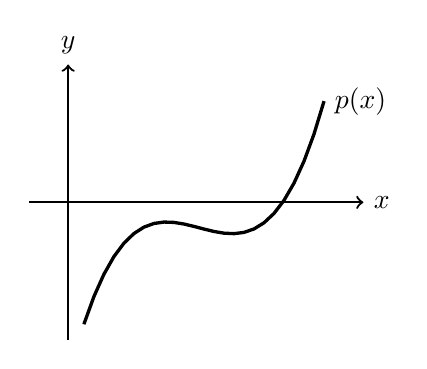
\begin{tikzpicture} [scale = 1]
\draw[->, thick] (-0.5,0) -- (3.75,0) node[right] {$x$};
\draw[->, thick] (0,-1.75) -- (0,1.75) node[above] {$y$};
\draw[very thick, domain=0.2:3.25] plot (\x,{(0.8*\x)^3 - 4*(0.8*\x)^2 + 5*(0.8*\x) - 2.25}) node[right] {$p(x)$};
\end{tikzpicture}
\end{columns}

\end{frame}

\begin{frame}{Newton's Method}

\begin{columns}
\column{0.5\textwidth}
\begin{itemize}
    \item Initial guess $x_0$.
    \item Requires its derivative.
    \item Rule: $x_{i+1} = x_i - \frac{f(x_i)}{f'(x_i)}$.
    \item Divide by zero problem.
    \item Called an \textit{Open method}.
\end{itemize}


\column{0.5\textwidth}
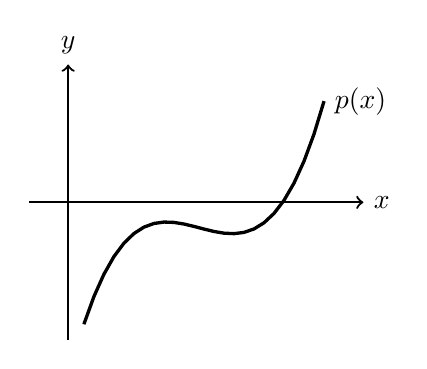
\begin{tikzpicture} [scale = 1]
\draw[->, thick] (-0.5,0) -- (3.75,0) node[right] {$x$};
\draw[->, thick] (0,-1.75) -- (0,1.75) node[above] {$y$};
\draw[very thick, domain=0.2:3.25] plot (\x,{(0.8*\x)^3 - 4*(0.8*\x)^2 + 5*(0.8*\x) - 2.25}) node[right] {$p(x)$};
\end{tikzpicture}
\end{columns}

\end{frame}

\begin{frame}
\begin{figure}[h]
    \centering
    \includegraphics[width=0.75\linewidth]{newpolynomial.png}
    \caption{$p(x) = x^6 - 2x^5 - 3x^4 + 4x^3 + 5x^2 + x - 7$ with bracket $[1, 1.5]$ and initial guess $x_0=-1.75$.}
\end{figure}
\vspace{-10pt}
\begin{itemize}
    \item Method behaviour.
    \item Descartes' rule of signs as a tool.
\end{itemize}
\end{frame}

\begin{frame}{Example of a Difficulty: Flat Regions}

\begin{figure}
    \centering
    \includegraphics[width=0.9\linewidth]{flatroot.png}
    \caption{$p(x) = (x-5)^9$ with bracket $[-5, 22]$ and initial guess $x_0 = 20$}
\end{figure}
\vspace{-10pt}
\begin{itemize}
    \item Performance: number of iterations and absolute error.
    \item Bracketed methods vs. Open methods.
    \item Specifics of the problem matter.
\end{itemize}
\end{frame}

\begin{frame}{Wilkinson's Polynomial}
    \[w(x) = \prod_{i=1}^{20}(x-i) = (x-1)(x-2)(x-3)\cdots(x-20)\]
    \begin{itemize}
        \item Example of a \textit{test polynomial}.
        \item Variety of roots found: $9, 7, 9, 13, 12, 13$.
        \item Open method initial guesses less than 0 generally find $x=1$.
        \item Limit to 15 iterations and plot the absolute error for various initial guesses less than zero.
    \end{itemize}
\end{frame}

\begin{frame}

\begin{figure}[h] \centering
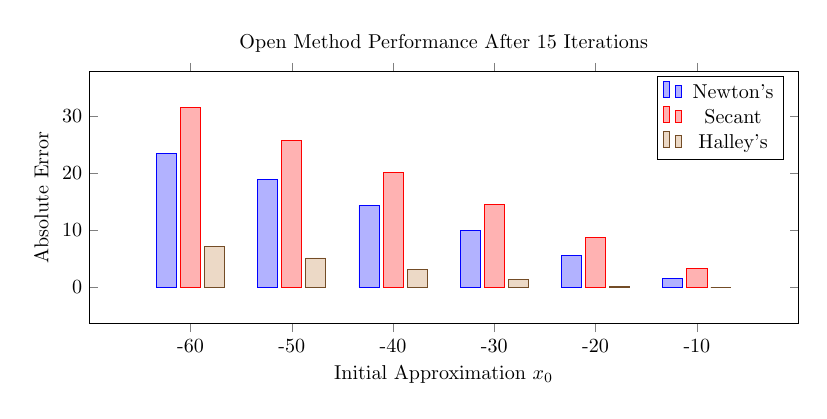
\begin{tikzpicture}[scale = 0.725]
\begin{axis}[ybar, 
enlargelimits=0.2,
width=14cm,
height=6cm,
title={Open Method Performance After 15 Iterations},
xlabel={Initial Approximation $x_0$},
ylabel={Absolute Error},
symbolic x coords={-60,-50,-40,-30,-20,-10},
xtick=data,
]
\addplot coordinates {(-60,23.5) (-50,18.9) (-40,14.4) (-30,9.96) (-20,5.57)  (-10,1.521)};
\addplot coordinates {(-60,31.6) (-50,25.8) (-40,20.2) (-30,14.5) (-20,8.82)  (-10,3.384)};
\addplot coordinates {(-60,7.23) (-50,5.19) (-40,3.23) (-30,1.43) (-20,0.117) (-10,0)};
\legend{\ Newton's,\ Secant,\ Halley's}
\end{axis}
\end{tikzpicture}
% \caption{Absolute error of various root-finders based on $x_0$ for the Wilkinson polynomial and known root $x=1$.}
% \label{errorplot}
\end{figure}

Linear approximations (for $-60 \le x_0 \le -10$):
\begin{align*}
    E_N(x_0) &\approx -0.44x_0 -2.87, \\
    E_S(x_0) &\approx -0.56x_0 -2.26.
\end{align*}

\end{frame}

\begin{frame}{Conclusion}
    \begin{itemize}
        \item Able to explain why the bisection method must converge and Newton's method often struggles with flat regions.
        \item Promising results for TOMS748 and Halley's method.
        \item We observed that there is no usual ``best'' method, as each has the potential to outperform the others depending on the specifics of the problem and polynomial.
        \item Future research: 
        \begin{itemize}
            \item High multiplicity roots next to each other,
            \item Functions other than polynomials, and
            \item Developing or modifying techniques.
        \end{itemize}
    \end{itemize}
\end{frame}

\end{document}